Let $\Omega \subset \R^d $ be a convex bounded domain.
First of all we repeat the basis definitions for the analysis of partial differential equations as they are introduced for example in \cite{Evans1998}.
\begin{definition}[Partial Differential Equation]
 A \emph{partial differential equation} (PDE) of order $k\in \N$ is an expression of the form
\begin{align}
	F(D^k(u(x)), D^{k-1}(u(x)), Du(x), u(x), x) = 0, \label{eq:general PDE}
\end{align}
where $F$ is given and $u$ is unknown.
\end{definition}
We focus in thesis on second order PDEs for our main PDE the \MA equation is of second order. Next to the order there exist further properties to categorise PDEs
\begin{definition}[Categories of PDEs]
	Given functions $a_{\alpha} $ and $f$ a PDE is called
	\begin{enumerate}
		\item \emph{linear} if it can be written in the form
		\[
			\sum_{|\alpha| \leq k} a_{\alpha} (x) D^{\alpha} u = f(x).
		\] 
		
		\item \emph{semilinear} if it can be written in the form
		\[
			\sum_{|\alpha| = k} a_{\alpha}(x) D^{\alpha} u + a_0(D^{k-1}u, Du, u, x)= f(x),
		\]	
		i.e. a semilinear PDE is nonlinear in the unknown function, but linear in the all partial derivatives.
		
		\item \emph{quasilinear} if it can be written in the form
		\[
			\sum_{|\alpha| = k} a_{\alpha}(D^{k-1}u, Du, u, x) D^{\alpha} u + a_0(D^{k-1}u, Du, u, x)= f(x),
		\]	
		i.e. a quasilinear PDE is nonlinear in (at least) on lower derivate, but linear in the highest order derivates.
		
		\item \emph{fully nonlinear}, if it depends nonlinearly upon the highest order derivatives.
	\end{enumerate}
	\todo{roman enumeration}
\end{definition}
A famous example for linear PDEs is the \emph{Poisson equation} $-\triangle u = f$, a semilinear PDE is for example the \emph{nonlinear Poisson equation} $-\triangle u = f(u)$. A well-known example for quasilienar PDEs are equations of the type $\nabla \cdot (A(u) \nabla u) = f$, where $A: \R^d \rightarrow \R^{d \times d}  $. The\MA equation $\mydet {D^2 u} = f$ which we will disuss later in detail is part of the last category, the nonlinear PDEs. 

Another important classification of second order PDEs is the ellipticity. 
\begin{definition}[Elliptic PDE{, \cite[p.207]{FGN2013}}]
	A fully nonlinear second order PDE is called \emph{elliptic} if its operator satisfy
	\begin{align}
		F(A,p,z,x) \leq F(B,p,z,x) \label{eq: ellipitic PDE}
	\end{align}
for all $x \in \Omega, z \in \R, p \in \R^d$ and $A,B \in \R^{d \times d}_{sym}$  with $A-B$ positive definite.
\end{definition}

A function $u$ fulfilling \eqref{eq:general PDE} is called a classical solution of the PDE. There are problems such that no such solution exists, often the demand on the high derivatives cannot be fulfilled. To admit less regular solutions one aims for a weaker solution notion. To do this one needs to we specify some spaces where weaker solutions could be contained.

\section{Functional Spaces}
According to the literature we refer by $W^{s,p}(\Omega)$ to the H\"older space, a set consisting of all $L^p(\Omega)$ functions whose distributional derivates up to order $s$ are contained in $L^ p(\Omega)$.
\todo{what is a distributional derivates}

Let $\triang$ be a shape regular, quasi-uniform simplicial triangulation of $\Omega$, for simplicity reasons we assume that $\triang$ consists only of triangles. We divide the edges $\edges$ into the subsets $\edgesi$ and $\edgesb$ containing all interior edges and boundary edges, respectively. On this basis we define the piecewise spaces
\begin{definition}[Piecewise Spaces]
The to the mesh associated spaces are
\begin{align}
	H^s(\triang) = \Pi_{T\in \triang}  H^s(T), W^{s,\infty}(\Omega) = \Pi_{T\in \triang} W^{s,\infty}(T).
\end{align}	
\end{definition}
\begin{definition}[Piecewise Polynomial Spaces] \label{def: piecewise polySpace}
	Further we denote the finite-dimensional space of piecewise polynomials by
\[	
	\mathcal P^k_h = \{ f \in L^\infty(\Omega); f \arrowvert_T \textnormal{ is a polynomial of (total) degree } \leq k \textnormal{ for every } t \in \mathcal T_h\}.
\]
\end{definition}

\todo{norms}
We use a subscript $h$ to indicate a piecewise evaluation/interpretation. Subsequently differential operators with a subscript $h$ imply separate differentiations on every triangle.

\section{Notation}
To formulate a method capable of discontinuities along triangle edges we need some edge operators.   

\begin{definition}[Edge Operators]
We denote the \emph{normal jump} of  a piecewise smooth function $u_h$ across an edge $e \in \edges$ by
\begin{align*}
	\llbracket u_h \rrbracket &= u_h^+ \cdot n^+ + u_h^-\cdot n^-  &&\text{ if } \partial T^+ \cap \partial T^- = e, \\
	\llbracket u_h \rrbracket &= u_h \cdot n  &&\text{ if } \partial T \cap \partial \Omega = e,
\end{align*}
where $n^\pm$ are the outward unit normals of $T^\pm$ and  $u_h^\pm(x) = \lim_{\varepsilon \rightarrow 0} u_h(x-n^\pm \varepsilon)$.

The \emph{average} of a piecewise smooth function $u_h$ across an edge $e \in \edges$ is defined by
\begin{align*}
	\laverage u_h \raverage &= \frac 1 2 \left(u_h^+ + u_h^-\right) &&\text{ if } \partial T^+ \cap \partial T^- = e, \\
	\laverage u_h  \raverage &= u_h &&\text{ if } \partial T \cap \partial \Omega = e,
\end{align*}
\end{definition}

Note, that the jump of a scalar is a vector, whereas the jump of a vector is a scalar.


\section{Finite Element Method}
Before we handle the \MA equation we recall how a finite element method works using the example of the general Poisson equation. 

%\subsection{The Poisson Problem}

\begin{definition}[Generalised Poisson Problem]
The \emph{Generalised Poisson Problem} is finding a function $u$ such that 
\begin{align}
	-\nabla \cdot (A \nabla u) = f \qquad &\text{ in }\Omega \label{eq: poisson eq} \\
	u = g \qquad &\text{ on } \partial \Omega    \label{eq: poisson bc}
\end{align}
for $ A:\R^d \rightarrow \R^{d \times d}$ symmetric and functions $f,g $. 
\end{definition}

We can set up a weak formulation based on variational principles.

Due to the main theorem of variation analysis every solution to \eqref{eq: poisson eq} is equivalent to 
\begin{align}
	-\int_\Omega \varphi \nabla \cdot (A \nabla u) = \int_\Omega \varphi f \qquad \forall \varphi \in C^\infty(\Omega).
\end{align}
Integration by parts yields to
\begin{align}
	\int_\Omega \nabla \varphi  \cdot A\nabla u -\int_{\partial \Omega} \varphi (A\nabla u) \mathbf{n}  = \int_\Omega \varphi f \qquad \forall \varphi \in C^\infty(\Omega). \label{eq: FE integration by parts}
\end{align}
\begin{definition}[Weak Solution]
	Functions satisfying \eqref{eq: FE integration by parts} are called \emph{weak solutions} of \eqref{eq: poisson eq}.
\end{definition}
The generalised poisson problem is well-posed in the sensse that it has a unique weak solutions for $A$ positive definite and $f\in L^2(\Omega)$, for a detailed analysis we recommend \cite[Chapter~6]{Evans1998}.

On the left-hand side in \eqref{eq: FE integration by parts} now only first derivatives of $u$ appear.
The main idea of the finite element method is to restrict the two spaces, namely the spaces where $\varphi$ and $u$ are come from to finite dimensional spaces $\Phi_h$ and $V_h$ of $C^\infty(\Omega)$.\\
The limited space $\Phi_h$ is called \emph{test space} and its inhabitants :) are called \emph{test functions}. $V_h$ is referred as \emph{ansatz} or \emph{trial space},  the contained functions accordingly \emph{ansatz} or \emph{trial functions}. To assert the boundary condition \eqref{eq: poisson bc} we demand $u_h|_{\partial \Omega} = g$ for every $u_h \in V_h$.

As the subscript $h$ suggests the two spaces normally are based on a triangulation $\triang$ such that every function is at least piecewise smooth. Consequently, the differential operators must be replaced by to $\Phi_h \cup V_h$ extended forms.

All in all the finite element methods searches for $u_h \in V_h$ such that 
\begin{align}
	\int_\Omega \nabla_h \varphi  \cdot A\nabla_h u_h -\int_{\partial \Omega} \varphi  \cdot (A\nabla_h u_h) \mathbf{n}  = \int_\Omega \varphi f \qquad \forall \varphi \in \Phi_h. \label{eq: weak formulation fe}
\end{align}

To construct $u_h$ we first choose a basis $B_{\Phi}$ of $\Phi$ and a basis $B_V$ of $V_h$.
Since the left-hand side is linear in $\varphi$ we only need to check the equations in \eqref{eq: weak formulation fe} for all $\varphi \in B_{\Phi}$. Exploiting also the linearity in $u_h$  we are able to reformulate the equations using approriate bilinear forms:
\begin{align}
	a(\varphi,u_h)  =b(\varphi) \qquad \forall \varphi \in \Phi_h. \label{eq: weak formulation fe bilinear}
\end{align}
for $a(v,w)= \int_\Omega \nabla_h v  \cdot A\nabla_h w -\int_{\partial \Omega} v (A\nabla_h w)\mathbf{n}$ and $b(v) = \int_\Omega v f$.\\
\todo{ueberarbeiten} Using basic linear Algebra we can rewrite \eqref{eq: weak formulation fe bilinear} as a linear system of equations $A \mathbf{u} = \mathbf{b}$ where  $\mathbf{u}$ is the coefficient vector of $u_h$ to the basis $B_V$.  

Typically the spaces $\Phi_h$ and $V_h$ are chosen to be piecewise polynomials which have support only on a few triangles. Thus, the spaces are easy to handle and the resulting linear system is sparse.
Choosing $\Phi_h = V_h$ yields to the \emph{Galerkin methods}.

\section{Discontinuous Galerkin (DG)} \label{sec: SIPG}
A recent idea is to choose the test and ansatz spaces to include discontinuous functions (even though the solution is expected to be smooth)\todo{kommentar sinnvoll}.
The main issue is the handling of derivatives along discontinuities.
\todo{DG mit numerischen Flux oder mehr wie TICAM?}

We recall our triangulation $\mathcal{T}_h$ of $\Omega$. We are able to use $\mathcal V_h = \mathcal P_h^k$ as defined in \ref*{def: piecewise polySpace} for the ansatz and test space in a finite element method, if we modify the procedure a bit: Due to the discontinuities along edges we perform the integration by parts in \eqref{eq: FE integration by parts} piecewise on every triangle leading to
\begin{align}
	a(\varphi, v) = & \sum_{T \in \triang} \int_T \nabla \varphi \cdot A \nabla v - \sum_{T \in \triang} \int_{\partial T} \varphi A \nabla v \cdot \mathbf n.
\end{align}
Since two adjacent elements share the same edge only with opposite normal vectors we can rewrite the middle term by
\begin{align*}
\sum\limits_{T \in \triang}\int_{\partial T} \varphi A \nabla v \cdot \mathbf n 
= &\sum\limits_{e \in \edgesi}\int_{e} \left( \varphi^+ A^+ \nabla v^+ \cdot \mathbf n^+ - \varphi^- A^- \nabla v^- \cdot \mathbf n^- \right) \\
& + \sum\limits_{e \in \edgesb}\int_{e} \varphi A \nabla v \cdot \mathbf n,
\end{align*}
where $x^\pm $ is $x$ evaluated in one of the two adjadecent elements $T^\pm$. With the identity $\mathbf n^- = -\mathbf n^+$ and formula $ac-bd = \frac 1 2 (a+b)(c-d) + a\frac 1 2(c+d)-b\frac 1 2(c+d)$  we get
\begin{align*}
	&\varphi^+ A^+ \nabla v^+ \cdot \mathbf n^+ - \varphi^- A^- \nabla v^- \cdot \mathbf n^+ \\
	= & \phantom{+} \frac 1 2 \left(\varphi^+ + \varphi^- \right) \left(A^+ \nabla v^+ \cdot \mathbf n - A^- \nabla v^- \cdot \mathbf n \right) \\
  &+  \varphi^+ \frac 1 2  \left(A^+ \nabla v^+\right) \cdot \mathbf n^+ - \varphi^- \frac 1 2 \left(A^- \nabla v^-\right) \cdot \mathbf n^+ \\
  = &  \jump {\average \varphi  A \nabla v}+ \jump {\varphi \average{ A \nabla v}}
\end{align*}
Therefore the weak formulation can be written as $a(v,\varphi) = l(\varphi)$ with 
\begin{align*}
  a(v, \varphi) = & \sum\limits_{T \in \triang} \int_T \nabla \varphi \cdot \left(A \nabla v\right) \\
	& - \sum\limits_{e \in \edgesi}\int_{e} \left( \jump {\average \varphi A \nabla v} + \jump {\varphi \average{ A \nabla v}} \right)\\
& - \sum\limits_{e \in \edgesb}\int_{e} \varphi A \nabla v \cdot \mathbf n
\end{align*}
and
\[
l(\varphi) = \sum_{T \in \triang} \int_T v f
\]
Due to the smoothness of $u$ and $w$ we can neglect the jump in $A \nabla u$ and find
\begin{align*}
 a(v, \varphi) = & \sum\limits_{T \in \triang} \int_T \nabla \varphi \cdot \left(A \nabla v\right) %\\
	- \sum\limits_{e \in \edgesi}
	\jump{ \varphi \average{ A \nabla v}} %\right)
	\\
& - \sum\limits_{e \in \edgesb}\int_{e} \varphi A \nabla v \cdot \mathbf n.
\end{align*}

Symmetrising our bilinear form $a$ by adding terms on both sides we have
\begin{align}
 a_S(v, \varphi) = &\sum\limits_{T \in \triang} \int_T \nabla \varphi \cdot A \nabla v \nonumber \\
  &-\sum\limits_{e \in \edgesi}\int_{e} \jump {\varphi \average{A \nabla v} }
 - \sum\limits_{e \in \edgesi}\int_{e} \jump{ v \average{ A \nabla \varphi}} \nonumber\\ 
 & - \sum\limits_{e \in \edgesb}\int_{e} \varphi A \nabla v \cdot \mathbf n 
    - \sum\limits_{e \in \edgesb}\int_{e} v A \nabla \varphi \cdot \mathbf n.
\end{align}
and 
\begin{align}
	l(\varphi) =& \sum\limits_{T \in \triang} \int_T \varphi f -\sum\limits_{e \in \edgesb}\int_{e} u_0 A \nabla \varphi \cdot \mathbf n.
\end{align} 

%and $f$
%\begin{align}
%	f_S(v,\varphi) = && \sum\limits_{T \in \triang} \int_T \varphi f \\
%	 				&+ &\sum\limits_{e \in \edgesb}\int_{e} \varphi \cof(D^2 w) \nabla v \cdot n \\
% &+ &\sum\limits_{e \in \edgesi}\int_{e} v \llbracket \cof(D^2 w) \nabla \varphi \cdot n\rrbracket \\
%	&-  &\sum\limits_{T \in \triang} \int_T v (\nabla \cdot \cof(D^2w)) \cdot \nabla \varphi \\
%\end{align} 

To enforce stability we enforce the following penalty terms [TICAM report 3.2.2.]
\begin{align}
	J^\sigma(\varphi, v) = \sum\limits_{e \in \edges} \int_e \frac \sigma {|e|} \jump \varphi \jump v \textnormal{ and } 	J^\sigma_0(\varphi, v) = \sum\limits_{e \in \edgesb} \int_e \frac \sigma {|e|} \varphi u_0  
\end{align}

Thus, we end up with the problem finding $v \in V_h$ such that
\[
	a_S(\phi,v) + J^\sigma(\varphi,v) = l(\varphi) + J^\sigma_0(\varphi)
\] 
$  \textnormal{for all } \varphi \in V_h$\

Just like in the finite element method we can derive a linear system of equations $A \mathbf{u} = \mathbf{b}$ with $A$ sparse and $\mathbf{u}$ representing the coefficient vector of $u_h$ to the basis $B_V$.  

\section{Implementation of a DG Method}
\todo{ Kommentar zur Implementation wegen Vorzeichen für Kantenterme}
To evaluate the integrals in the bilinearform  numerically an integration scheme is needed. Usually Gauss quadrature is the method of choice. Since ansatz and test functions are chosen to be piecewise polynomials a Gauss quadrature already is exact for only a few quadrature points.
Hence, the data we have to provide to assemble the sparse matrix $A$ are the gradient, the normal derivatives, i.e. $\nabla u \cdot \mathbf{n}$ and the function values of all test functions at each quadrature point.

To reduce the storage space one usually specify a reference cell $T_{ref}$ such that every triangle $T \in \triang$ is the image of $T_{ref}$ under an affine transformation $\Phi_T$. 
%We make use of the triangle spanned by the points $(0,0)^t, (0,1)^t$ and $(1,0)^t$ for our reference cell. 
Since the DG spaces also allow discontinuous functions choosing a polynomial basis $p^1_{ref},\dots,p^n_{ref}$ of $T_{ref}$ also induces a basis on every $T$, namely the basis consisting of 
\[
	p_T^i(x) = p^i_{ref}(\Phi_T^{-1}(x)), \qquad x \in T, 1 \leq i \leq n.
\]
%Hereafter the only polynomials we refer to are the ones given in this basis.
Knowing $\Phi_T$ and the reference cell $T_{ref}$ most required data on a triangle $T$ can be easily derived. We explain how to do that in detail for the two-dimensional case.

\begin{example}
From now an we consider $\Omega \subset \R^2$ and we choose the reference triangle to be the triangle spanned by the points $\point 0 0, \point 0 1$ and $\point 1 0$.
Suppose we want to figure out the transformation for the triangle $T = \langle v_1,v_2,v_3 \rangle$.
It has to hold
\[
\Phi\left(\point 0 0\right) = v_0, \Phi\left(\point 0 1\right) = v_1 \textnormal{ and } \Phi\left(\point 1 0\right) = v_2
\]
Since every two-dimensional affine transformation has the form $\Phi(x) = Ax+b$ for $A \in \R^{2 \times 2}$ and $b \in \R^2$ it is easy to verify that we have $A = \begin{pmatrix} v_1-v_0 & v_2-v_0\end{pmatrix}$ and $b = v_0$.
Having determined the transformation we are able to easily calculate its inverse $\Phi_T^{-1}(x) = A^{-1} (x-b) =: A^{-1} x- \tilde b$. \\
Let $x \in T$ have the barycentric coordinates $\beta_0, \beta_1$ and $\beta_2$, then because of $\Phi^{-1}$'s linearity we find
\begin{align*}
	p^i_T(x) =& p_T^i( \beta_0 v_0 +\beta_1 v_1 + \beta_2 v_2  ) \\
	=& p^i_{ref}(\Phi_T^{-1}(\beta_0 v_0 +\beta_1 v_1 + \beta_2 v_2)) \\
	=& p^i_{ref}(\beta_0 \Phi_T^{-1}(v_0) +\beta_1 \Phi_T^{-1}(v_1) + \beta_2 \Phi_T^{-1}(v_2)) \\
		=& p^i_{ref}(\beta_0 \point 0 0 +\beta_1 \point 0 1 + \beta_2 \point 1 0 ), \qquad 1 \leq i \leq n.
\end{align*}
Thus, basis function values in $T$ can be simply determined by barycentric coordinates. From nows on we refer with $x_{ref}$  to the point $\beta_0 \point 0 0 +\beta_1 \point 0 1 + \beta_2 \point 1 0$ which is the to $x$ corresponding point in the reference triangle .

Similarly we can affiliate the determinant of the gradient in $T$ to a caculation in $T_{ref}$. With the chain rule we have
\begin{align*}
	\left(\nabla_x p_T^i(x)\right)^t = D_x p)_T^i(x) =& D_x p^i_{ref}(\Phi_T^{-1}(x)) \\
	  =& D_{\Phi_T^{-1}(x)}p^i_{ref}(\Phi_T^{-1}(x)) \cdot D_x  \Phi_T^{-1}(x) \\
	  =& D_{x_{ref}}p^i_{ref}(x_{ref}) \cdot  A^{-1}
\end{align*}
and thus
\begin{align}
	\nabla_x p_T^i(x) = A^{-t} \cdot \nabla_{ref}(x_{ref}), \qquad 1 \leq i \leq n.
\end{align}

Analogous proceeding yields for the Hessian
\begin{align}
D_x^2p_T^i(x) = A^{-t} D_{x_{ref}}^2p^i_{ref}(x_{ref})  A^{-1}, \qquad 1 \leq i \leq n.
\end{align}

Concluding all information of a cell we need to store is the Jacobian of its transformation, i.e. $A$ and its normals. We are able to calculate all further information with the data provided by the reference triangle.
\end{example}

Imagine a typical mesh refinement our triangulation is created by refinement of a coarser mesh. We only to refer to a specific kind of refinement, namely given a triangulation $\triang$ dividing every triangle $T \in \triang$ into four to $T$ similar triangles as is shown in figure \ref{pic: refinement}. We denote the finer grid by $\triangFine$ for the diameter of each triangle is halved.

\begin{figure}[h]
\usetikzlibrary{calc}

		\begin{center}
		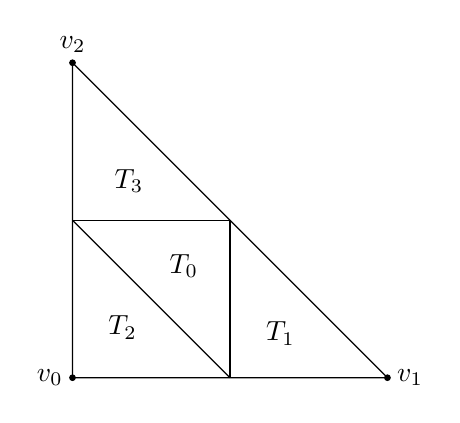
\begin{tikzpicture}
%define coordinates
			\coordinate (vEins) at (0,0) ;
			\coordinate (vZwei) at (0:4cm);
			\coordinate (vDrei) at (90:4cm);

%draw triangle
			\draw (vEins) -- (vZwei) -- (vDrei) -- cycle;

%draw refined triangle
			\draw ($(vEins)!0.5!(vZwei)$) -- ($(vEins)!0.5!(vDrei)$);
			\draw ($(vDrei)!0.5!(vZwei)$) -- ($(vEins)!0.5!(vDrei)$);
			\draw ($(vEins)!0.5!(vZwei)$) -- ($(vZwei)!0.5!(vDrei)$);

%draw nodes
			\draw[fill =black] (vEins) circle (1pt) node[left] {$ v_0$};
			\draw[fill =black] (vZwei) circle (1pt) node[right] {$v_1$};
			\draw[fill =black] (vDrei) circle (1pt) node[above] {$v_2$};

%			\draw node at (30:2.4cm) {$T_1$};

			\draw node at (45:0.9cm) {$T_2$};
			\draw node at (45:2cm) {$T_0$};
			\draw node at (74:2.6cm) {$T_3$};
			\draw node at (12:2.7cm) {$T_1$};

		\end{tikzpicture}
		\end{center}

\caption{Refinement of a triangle}
 \label{pic: refinement}
\end{figure}

We identifying the new triangles with the original cell $T$ calling it their basecell. Repeating the refinement we can relate a cell in the finest mesh with a basecell in the original triangulation.
The benefit of saving a base cell $T^T_b$ is that the transformation matrix of the transformation from $T^T_b$ is a diagonal matrix and that a it has the same, or for the innermost triangle opposite directed normals.
\todo{example as in fenics book p. 160 figure 8.1}

\begin{example}
In fact in the two-dimensional case the Jacobian of a transformation from the base cell to a $l$ times refined triangle is $
	\begin{pmatrix}
		\frac 1 {2^l} & 0 \\ 0 & \frac 1 {2^l}
	\end{pmatrix} \text{ or }
	\begin{pmatrix}
		-\frac 1 {2^l} & 0 \\ 0 & -\frac 1 {2^l}
	\end{pmatrix}$ respectively if there has be an odd number of ??? inner refinements\todo{ueberarbeiten}.

Hence, we have for a point $x \in T$
\begin{align}
\nabla_x p^i(x) &= \pm 2^l A^{-t} \cdot \nabla_{ref}(x_{ref}), \label{eq: trafo grad}\\
\nabla_x p^i(x) \mathbf n &= 2^l A^{-t} \cdot \nabla_{ref}(x_{ref}) \mathbf{ n_{b}} \qquad \text{ and } \\
D_x^2 p^i(x) &= 2^{2l} A^{-t} D_{x_ref}^2 p^i(x_{ref}), \qquad 1 \leq i \leq n,
\end{align}
where $l \in \N$ indicates how often $T$ is refined with respect to the original mesh, $A$ is the Jacobian of the transformation matrix to $T$'s base cell and $\mathbf n_b$ the to $n$ corresponding normal in the base cell. Note, that this even hold for the inner refined triangle since the minus sign in the Jacobian cancels with the minus sign of the with respect to the base cell opposite directed normal.
When evaluating the first part of the bilinearform, i.e. $\nabla \phi \cdot A \nabla v$ we see that for two basis polynomials $p_T^i, p_T^j$ having only support on $T$ the sign of the right-hand side in \eqref{eq: trafo grad} does not matter for both gradients have the same sign. Of course for other combinations of polynomials the terms always equals zero because the polynomials' suppose is chosen such that all other gradients vanish in the inner of $T$.
So, we are able to save a lot of memory if we store instead of the data at the quadrature points in all refined cells just the data of the base cell and the number of refinements. The refined cells contained in the actual mesh are referred as \emph{leaf cells}.
\end{example}

Another crux of the implementation are of course the face terms. 
Given that the support of each basis element is contained in one triangle, the contribution to the volume integrals can be calculated visiting the cell only once.
Face terms can be collected \todo{text from laptop}

\begin{algorithmic}
\Ensure every cell flag is false
\ForAll {cells} 
\State get cell data
\State calculate volume terms
	\ForAll {faces}
		\If {neighbour across the face exists} 
			\If {not neighbour flag}
					\State get neighbour cell data
					\State calculate face terms
			\EndIf
		\Else
			\State calculate boundary term
		\EndIf
\EndFor
	\State cell flag to true 
\EndFor
\State Reset every cell flag to false
\end{algorithmic}

While assembling the matrices each face has to be naturally processed only once. One has to take that the normal derivatives are stored always with respect to 
\todo{at the beginning difference face edge }

\newpage

To apply a DG method to more difficult PDEs such as the \MA equation we need some algebraic and analytic identities for the Hessian.
\section{Hessian Identities}

\begin{definition}[Cofactor Matrix] \label{def: cof matrix}
	The \emph{cofactor matrix} of a matrix $A \in \R^{d \times d}$ is defined by the entries
	\begin{align}
	(\mycof A )_{i,j} = (-1)^{i+j} \mydet{A_{ij}},
	\end{align}
	where $A_{ij}$ denotes the matrix resulting from deleting the $i$-th row and $j$-column in $A$.
\end{definition}

In the two-dimensional case the cofactor matrix of the hessian simplifies to
\begin{align}
\mycof {D^2 u} = \begin{pmatrix}
								\dxx{x_2} u & -\frac {\partial u}{\partial x_1 x_2} \\
								-\frac {\partial u}{\partial x_2 x_1} & \frac {\partial u}{\partial x_1^2} 
							\end{pmatrix}.
\end{align}


Very advantageous is the behaviour of the cofactor matrix of a hessian if a divergence is applied to it:
\begin{definition}[Matrix Divergence]
	$\nabla \cdot A$ for a matrix $A \in ?^{d \times d}$ is defined by taking the divergence row-wise,i.e.
\[
	\nabla \cdot A = \begin{pmatrix} \nabla \cdot A_1 \\ \vdots \\ \nabla \cdot A_d\end{pmatrix}
	= \begin{pmatrix} \sum_{j = 1}^{d} \dx{x_i} A_{1,j} \\ \vdots \\ \sum_{j = 1}^{d} \dx{x_i} A_{d,j}\end{pmatrix}.
\]
	
	\todo {ueberarbeiten}
\end{definition}

\begin{lemma}[Divergence-Free Property of Cofactor Matrices] \label{la: divergence free cof}
For smooth functions $u$ the cofactor matrix of the hessian is divergence-free:
\[
	\nabla \cdot \mycof{D^2 u} = 0.
\] 
\end{lemma}
\begin{proof}
\begin{align*}
	\nabla \cdot \mycof{D^2 u} = \sum_{i=1}^{d} \dx{ x_i}\mycof{D^2 u}_i = 
	\begin{pmatrix}
		\frac {\partial^3} {\partial x_1 {x_2}^2 } -\frac {\partial^3} {\partial{x_2} x_1 {x_2}} \\
				\frac {\partial^3} {\partial {x_1}x_2 {x_1}} -\frac {\partial^3} {\partial x_2 {x_1}^2 }
	\end{pmatrix}
\end{align*}
By Schwarz' theorem the latter equals zero if $u$ is thrice continuous differentiable.
\end{proof}


\begin{lemma}[Integration by parts for the Frobenius product] \label{la: integration by parts Frobenius}
For a Frobenius product with the hessian's cofactor matrix  the following integration by parts rule holds for smooth $u$
\[
	\int_\Omega (D^2 u : B) = - \int_\Omega (\nabla \cdot B) \cdot \nabla u + \int_{\partial \Omega}  B \nabla u \bf n
\] 
\end{lemma}

\begin{proof}
The proof is based on applying integration by parts row-wise
\begin{align*}
- \int_\Omega (\nabla \cdot B) \cdot \nabla u &= 
- \int_\Omega \sum_{i = 1}^{d} (\nabla \cdot B_i) \dx {x_i} u \\
&=  \int_\Omega \sum_{i = 1}^{d} B_i \cdot  (\nabla \dx {x_i} u) - \int_{\partial \Omega} \sum_{i = 1}^{d} (B_i) \dx {x_i} u \mathbf{n} \\
&=  \int_\Omega \sum_{i = 1}^{d}\sum_{j= 1}^{d} B_{ij} \dxy {x_i}{x_j} u- \int_{\partial \Omega} B \nabla u \mathbf{n} \\
&=  \int_\Omega (D^2 u : B)- \int_{\partial \Omega} B \nabla u \mathbf{n} 
\end{align*}
\end{proof}

When later talking about weak formulation it comes handy to have a divergence form of the latter 
\begin{lemma}[Divergence form of the Frobenius Product] \label{la: An application of the divergernce product rule}
\[
		\nabla \cdot \left( \mycof {D^2 u } \nabla v \right) %- \nabla \cdot \left(\mycof {D^2 u }\right) \nabla v
		= \mycof {D^2 u}: D^2 v
\] 
\end{lemma}


\begin{lemma}[Divergence-Free Property of Cofactor Matrices]
For the Frobenius product the following integration by parts rule holds
\[
	\nabla \cdot \mycof{D^2 u} = 0
\] 
\end{lemma}


\begin{lemma}[Integration by parts for the Frobenius product]
For the Frobenius product the following integration by parts rule holds
\[
	\int_\Omega (D^2 u : B) = - \int_\Omega (\nabla \cdot B) \cdot \nabla u + \int_{\partial \Omega}  B \nabla u \boldmath n
\] 
\end{lemma}

\begin{proof}
\begin{align*}
\nabla \cdot \left( \mycof {D^2 u } \nabla v \right) =&%- \nabla \cdot \left(\mycof {D^2 u }\right) \nabla =& 
\sum_{i= 1}^{d} \dx {x_i} 	\left( \sum_{j= 1}^{d} \mycof {D^2 u }_{i,j} \dx{x_j} v \right)\\
%&-  \sum_{j= 1}^{d}  \sum_{i= 1}^{d} \left(\dx {x_i} \mycof {D^2 u }_{i,j}  \right) \dx{x_j} v \\
=&  \sum_{i= 1}^{d} \sum_{j= 1}^{d}  \left(\dx {x_i} \mycof {D^2 u }_{i,j}  \right) \dx{x_j}v + \sum_{i= 1}^{d} \sum_{j= 1}^{d}  \mycof {D^2 u }_{i,j} \dxy{x_j}{x_i}v\\
=&  \sum_{j= 1}^{d}  \nabla \cdot \left(\mycof {D^2 u }\right)_j \dx{x_j}v + \sum_{i= 1}^{d} \sum_{j= 1}^{d}  \mycof {D^2 u }_{i,j} \dxy{x_j}{x_i}v\\
=&   \nabla \cdot \left(\mycof {D^2 u }\right) \nabla v+ \mycof {D^2 u }:D^2v
\end{align*}
The hypothesis results from the fact that the cofactor matrix of the hessian is divergence-free.
\end{proof}
